\section{Detekce objektů pomocí strojového učení}\label{sec:detekce-objektu-pomoci-strojoveho-uceni}

%todo zapracovat
%Tento model má již předučeno 80 kategorii, které umí v základní verzi detekovat.
%Mezi těmito kategoriemi je také pes.

\subsection*{Úvod do problematiky}\label{subsec:uvod-do-problematiky}
V posledních letech došlo k významnému pokroku v oblasti počítačového vidění, což umožňuje efektivní a přesné rozpoznávání objektů v různých prostředích.
Jednou z nejmodernějších knihoven, která si získala širokou popularitu, je YOLO11~\cite{ultralytics_yolo} (You Only Look Once version 11).
Tato knihovna přináší rychlé a přesné metody detekce objektů a je ideální pro implementaci v reálném čase.
V této sekci se zaměříme na to, jak využít YOLO11 ke specifickému úkolu: rozpoznávání slepic v kurníku.
Automatizované rozpoznávání umožňuje sledování počtu slepic.
Použití YOLO11 přináší následující výhody:

\begin{enumerate}
    \item Rychlost a přesnost - YOLO11 je navrženo pro rychlou detekci objektů s vysokou mírou přesnosti, což je ideální pro aplikování v reálném čase na farmách.
    \item Jednoduchost implementace - díky snadnému rozhraní a rozsáhlé dokumentaci je integrace YOLO11 do existujících systémů velmi přímočará.
    \item Flexibilita - můžete trénovat model na vlastním datasetu slepic, což zajistí optimální rozpoznávání i ve specifických podmínkách vašeho kurníku.
\end{enumerate}
V následujících sekcích si podrobně projdeme kroky, jak připravit dataset, trénovat vlastní model se zaměřením na rozpoznávání slepic a jak jej implementovat do našeho systému monitorování.

\subsection*{Obrázkový dataset}\label{subsec:obrazkovy-dataset}

Obrázkový dataset je strukturovaná kolekce obrazových dat, která se používá pro potřeby strojového učení a počítačového vidění.
Tyto datasety obsahují jednotlivé obrázky, které jsou často spojeny s dodatečnými informacemi nebo anotacemi, jež jsou potřebné pro trénink modelů.
Níže jsou uvedeny hlavní aspekty, které charakterizují obrázkové datasety:

\begin{enumerate}
    \item Obrázky - snímky, které mohou být v různých formátech (např. JPEG, PNG). Rozlišení a počet barev se může lišit v závislosti na účelu datasetu
    \item Anotace - metadata obsahující následující elementy
    \begin{itemize}
        \item Klasifikační štítky - identifikují, co se na obrázku nachází (např. „kočka“, „pes“, „slepice“)
        \item Ohraničující boxy - polohu specifických objektů na obrázku
    \end{itemize}
\end{enumerate}

Datasety jsou klíčové pro vývoj a zlepšování modelů strojového učení, protože poskytují potřebné tréninkové a testovací údaje.

V kontextu využití datasetů pro strojové učení je důležité zajistit, aby datasety byly kvalitní, rozmanité a dostatečně rozsáhlé, což pomáhá modelům převážně se zobecněním a výkonem v různorodých situacích.
Pro specifické nasazení v babičině kurníku jsem připravil vlastní dataset, který jsem použil pro doučení již existujícího základního modelu, který poskytuje Yolo11.
Záběry jsem vyfotil mobilem v prostředí babiččina výběhu a kurníku.
Existuje mnoho systémů pro tvorbu anotací (image labeling).
Já jsem zvolil Azure AI - Azure Machine Learning studio~\cite{aml}.
Pro práci je velmi intuitivní a nechá se spustit v několika krocích.
Nejdříve jsem pomocí průvodce vytvořil nový projekt jak je znázorněno na obrázku~\ref{fig:create_learning_project}.

\begin{figure}[H]
    \centering
    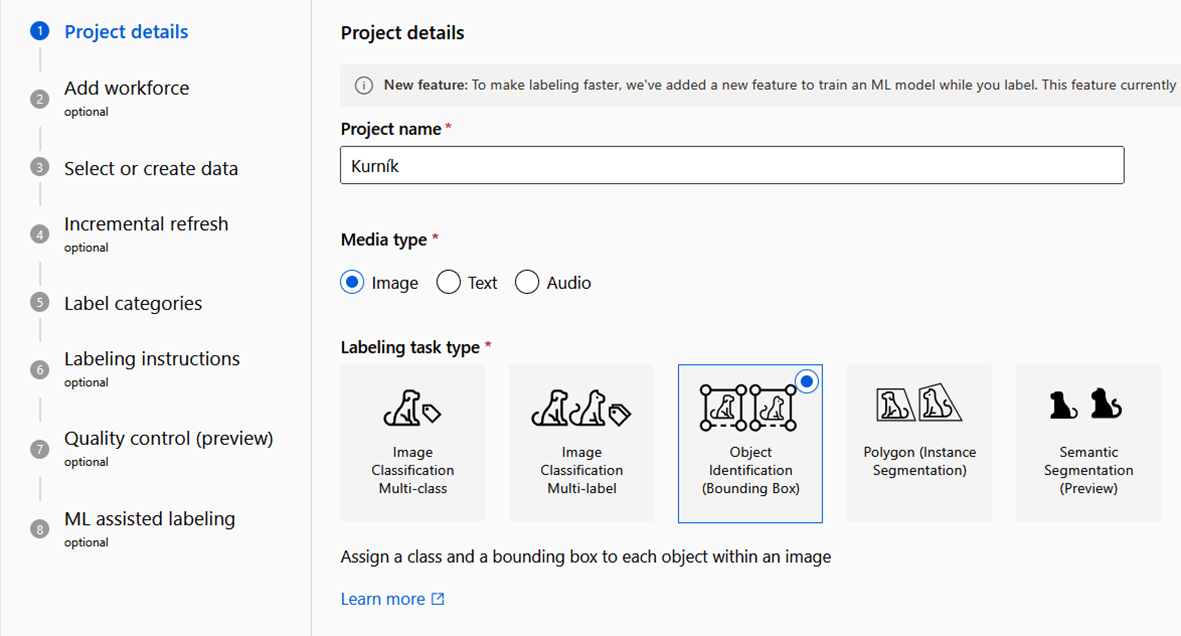
\includegraphics[width=1.0\textwidth]{img/create_learning_project}
    \captionAuthorSource{Vytvoření nového projektu v AML}
    \label{fig:create_learning_project}
\end{figure}


Dále jsem vybral zdroj obrázků, které bylo potřeba klasifikovat.
Vzhledem k tomu, že se jedná o cloudovou službu bylo třeba obrázky slepiček na Azure naimportovat.
Na obrázku~\ref{fig:dataset_selection} je snímek obrazovky z Azure Machine Learning studia, kde se zrovna dataset importuje.

\begin{figure}[H]
    \centering
    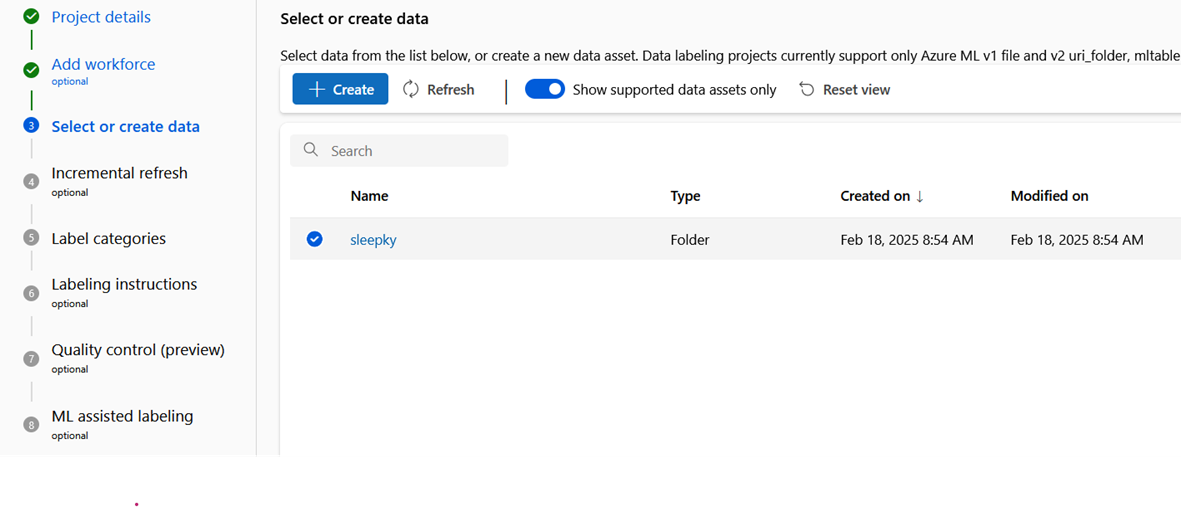
\includegraphics[width=1.0\textwidth]{img/dataset_selection}
    \captionAuthorSource{Tvorba datasetu v AML}
    \label{fig:dataset_selection}
\end{figure}

V dalším kroku jsem nadefinoval kategorie, které budu chtít v obraze identifikovat.
V mém případě jsem zvolil label „slepice“.
Definice kategorií je na obrázku~\ref{fig:category_definition}.

\begin{figure}[H]
    \centering
    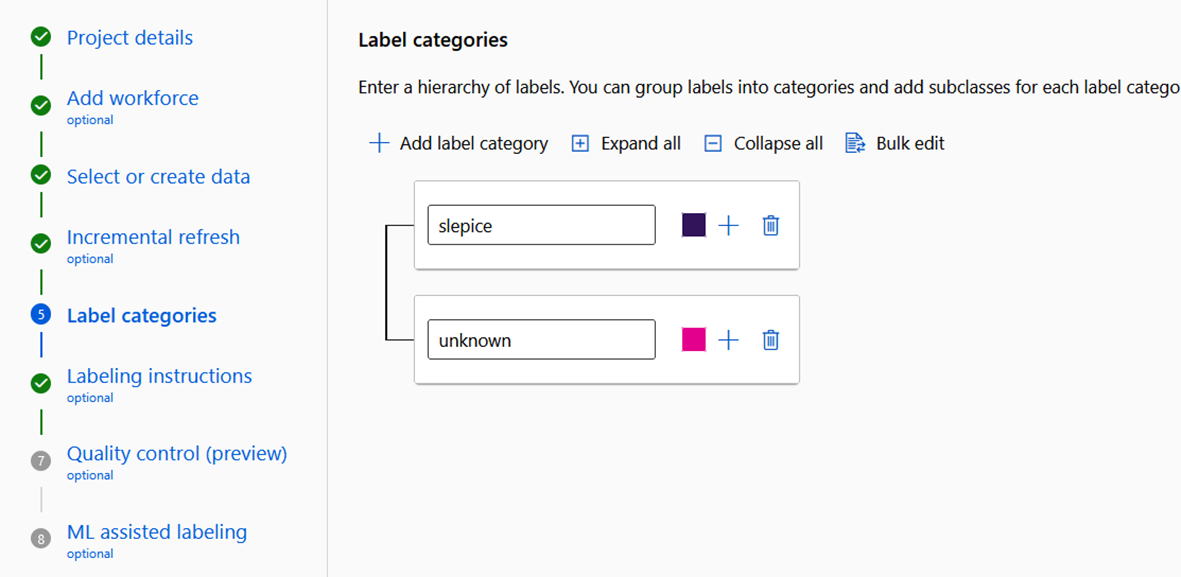
\includegraphics[width=1.0\textwidth]{img/category_definition}
    \captionAuthorSource{Definice kategorií pro učení v AML}
    \label{fig:category_definition}
\end{figure}

V následujícím kroku následovala nejméně zábavná činnost.
Bylo třeba projít jednotlivé snímky a ručně vybrat oblasti, kde já jako člověk vidím slepici.
Oblast, kterou jsem označil se pak následně ukládá jako metadata k~obrázku.
Tento proces je znázorněn na obrázku~\ref{fig:chicken_labeling}.

\begin{figure}[H]
    \centering
    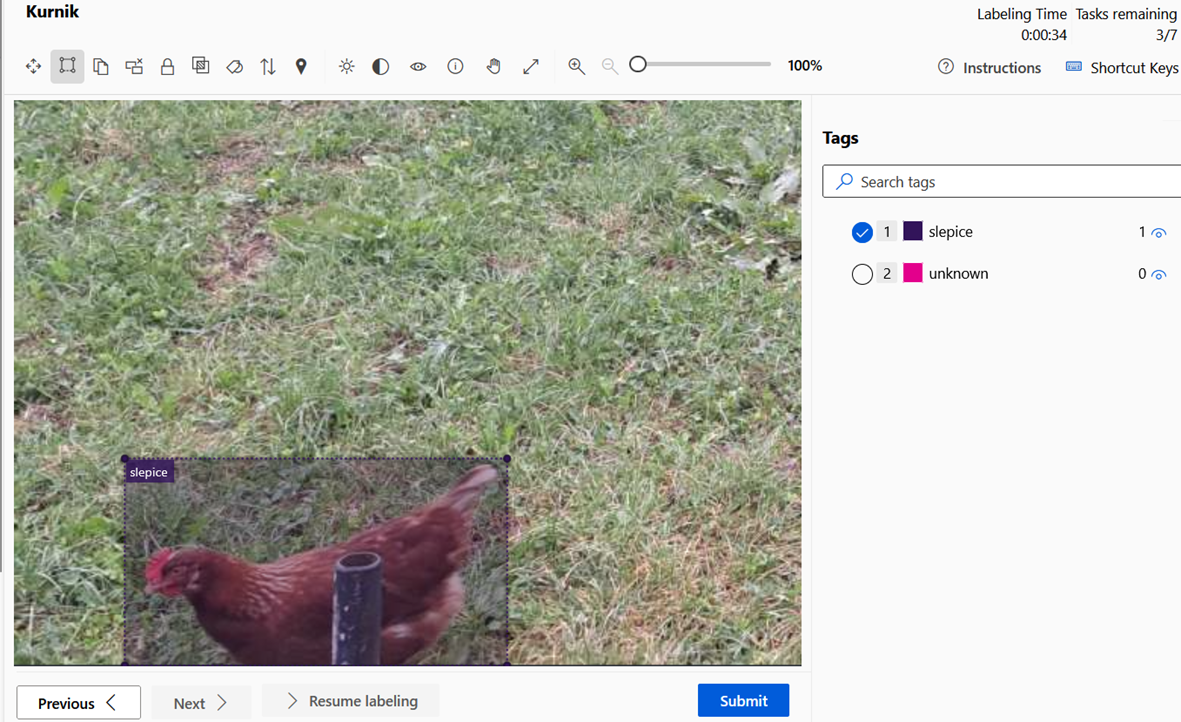
\includegraphics[width=1.0\textwidth]{img/chicken_labeling}
    \captionAuthorSource{Označování slepic pomocí AML}
    \label{fig:chicken_labeling}
\end{figure}

Když se podařilo projít celý obrázkový dataset, mohl jsem vyexportovat „labeling“ data.
Jak jsem psal výše, mít kvalitní učící dataset je důležité, proto jsem exportoval pouze data, která se podařilo úspěšně označit.
Do fotogalerie se mi dostalo i několik nejasných snímků, případně těch, kde slepice nebyla vůbec.
Takové snímky jsem vyřadil.
Anotace jsem exportoval ve formátu COCO~\cite{COCOFormat}~\ref{sec:coco_format}.
Formát COCO (Common Objects in Context) je standardní formát pro anotaci obrázků používaný ve strojovém učení a počítačovém vidění.
Jeho hlavním cílem je poskytnout strukturu pro uložení informací o objektech v obrázcích, což umožňuje efektivní trénink a hodnocení modelů detekce objektů, segmentace a dalších úloh počítačového vidění.
Obrázek~\ref{fig:create_learning_project} ukazuje, jak například může vypadat nastavení pro export COCO formátu z AML.

\begin{figure}[H]
    \centering
    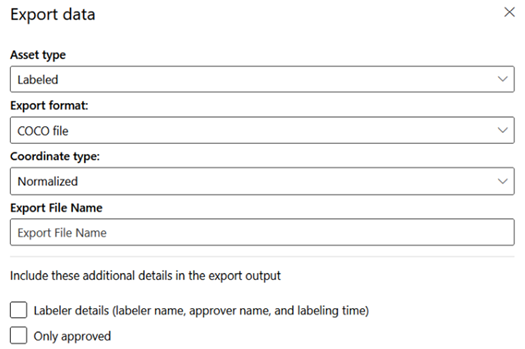
\includegraphics[width=1.0\textwidth]{img/export_coco_format}
    \captionAuthorSource{Export metadat k obrázkům z AML do COCO formátu}
    \label{fig:export_coco_format}
\end{figure}

Soubor obsahuje několik klíčových sekcí: images, annotations, a categories.\newline
Zde je popis jednotlivých částí daného JSON souboru ve formátu COCO:
\begin{enumerate}
    \item images: Tato sekce obsahuje informace o každém obrázku v datasetu
    \begin{itemize}
        \item id - unikátní identifikátor obrázku (zde 1)
        \item width a height - rozměry obrázku (zde 534 pixelů x 291 pixelů)
        \item file\_name: cesta k souboru obrázku včetně názvu souboru
        \item coco\_url, absolute\_url - adresy, kde je obrázek uložen, ať už v cloudovém sandboxu (coco\_url) nebo přes URL pro přímý přístup (absolute\_url)
        \item date\_captured - čas a datum zachycení obrázku v UTC formátu
    \end{itemize}
    \item annotations - poznámky k jednotlivým objektům na obrázcích
    \begin{itemize}
        \item id - unikátní identifikátor anotace (zde 1)
        \item category\_id - odkazuje na kategorii objektu
        \item image\_id - ID obrázku, na který se tato anotace vztahuje
        \item area - relativní plocha objektu na obrázku (zde 0.016)
        Tato hodnota je často normalizována vzhledem k velikosti obrázku
        \item bbox - relativní souřadníce (bounding box)
    \end{itemize}
    \item categories - seznam kategorií, do kterých mohou objekty na obrázcích patřit
    \begin{itemize}
        \item id - unikátní identifikátor kategorie
        \item name - jméno nebo popis kategorie (zde "slepice" a "unknown")
    \end{itemize}
\end{enumerate}

Tento JSON tedy popisuje dataset obsahující obrázek s jedním označeným objektem, který patří do kategorie "slepice".
COCO formát umožňuje uložení komplexních a strukturovaných dat o objektech na obrázcích, což je velmi užitečné pro trénování a testování modelů strojového učení.
Příklad tohoto formátu metadat pro strojové učení je na obrázku~\ref{fig:coco_format}.

\begin{figure}[H]
    \centering
    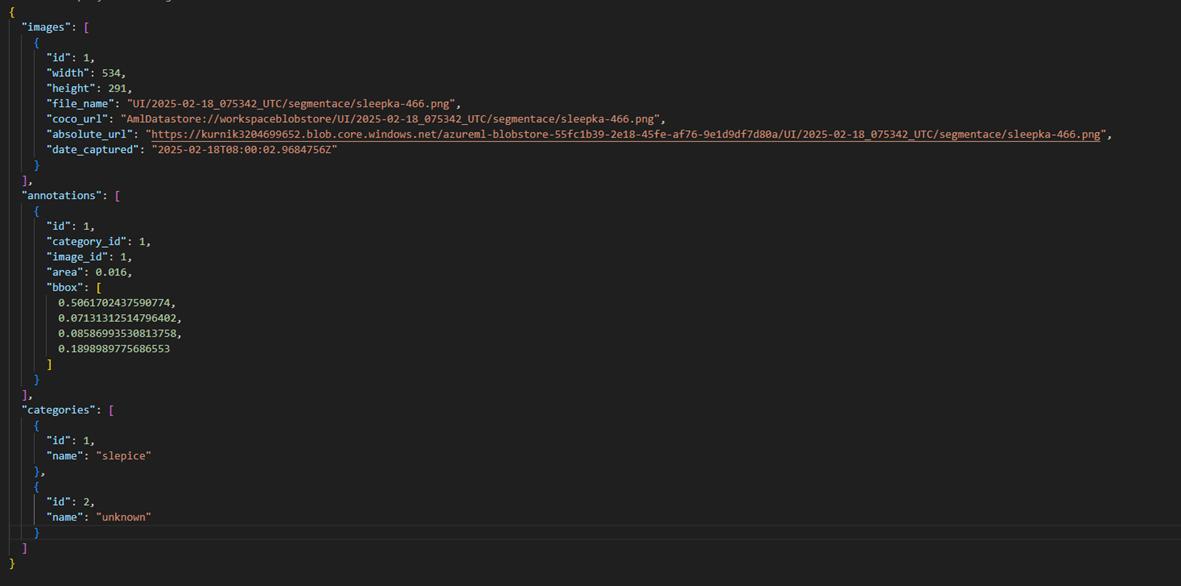
\includegraphics[width=1.0\textwidth]{img/coco_format}
    \captionAuthorSource{Ukázka COCO metadat pro učení}
    \label{fig:coco_format}
\end{figure}

\subsection*{Doučování modelu Yolo11}\label{subsec:doucovani-modelu-yolov11-o-novou-tridu}
V předchozí sekci jsem si popsali, jak vytvořit zdroje dat a nyní jsme připraveni vyučit existující model.
Doučovat doma existující model je relativně složité, ale díky výborné dokumentaci na stránkách Ultralytics.com~\cite{ultralytics_yolo} jsem to zvládnul.
Základem pro úspěšné a efektivní učení je hardware.
Hlavně GPU, protože trénování modelů hlubokého učení je výpočetně náročné.
Vypozoroval jsem, že největší vliv na učení má velikost paměti grafické karty.
V mém případě byla použita Nvidia RTX 4070.
O stavbě a následném učení neuronových sítí by se nechalo napsat desítky stránek, ale to není předmětem mojí práce.
Rád bych alespoň představil blokové schéma učícího procesu, který jsem použil.\newline
\newline
Pro učení jsem použil script, který jsem si připravil.
Volání jednotlivých kroků pro učení je znázorněno na screenshotu učící metody na obrázku~\ref{fig:learn_script}

\begin{figure}[H]
    \centering
    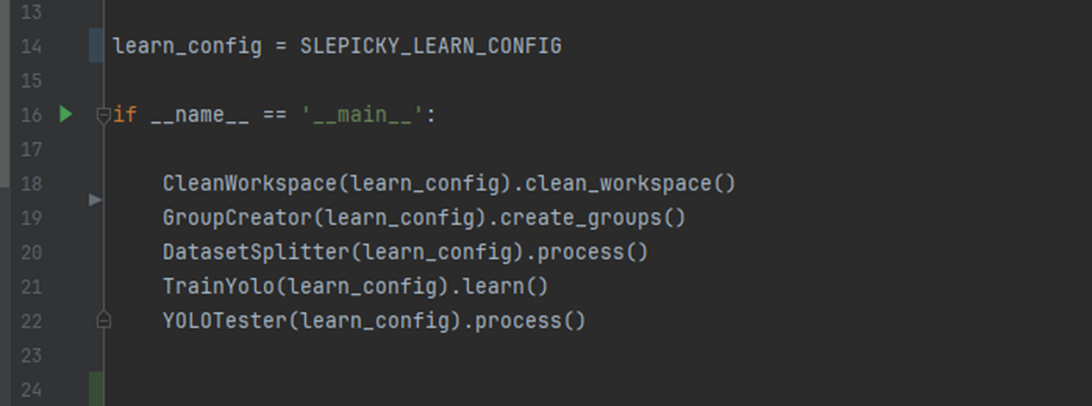
\includegraphics[width=1.0\textwidth]{img/learn_script}
    \captionAuthorSource{Kód pro učení nového modelu}
    \label{fig:learn_script}
\end{figure}

\subsubsection*{Krok 1 - CleanWorkspace}
Tento krok je zodpovědný za přípravu pracovního prostředí před zahájením tréninkového procesu.
Odstraňuji v něm archivaci stávajících dat a modelů, které mi ve workspace zůstaly z předchozích běhů a již nejsou potřebné.
Čištění pomáhá zabránit kolizím s předchozími seancemi a udržet v něm pořádek, což zajišťuje, že nové modely a datové soubory jsou aktuální a správně organizované.

\subsubsection*{Krok 2 - GroupCreator}

Tento krok se zaměřuje na organizaci dat do různých skupin pro trénování a testování modelu.
Data mám rozdělena v několika různých adresářích a tento krok má na starost jejich správné složení.
Stejná data používám pro výuku modelu na počítání slepic, detekce vetřelce a plánované reidentifikace slepic.

\subsubsection*{Krok 3 - DatasetSplitter}

Proces rozdělení datasetu je klíčový pro oddělení trénovací, validační a testovací sady.
Rozdělení může být prováděno v daných poměrech, například 70\% trénovací data, 15\% validační data a 15\% testovací data.
Správné rozdělení dat je důležité pro zajištění objektivního hodnocení modelu, aby se předešlo přeškolení.
Tento krok také zajišťuje, že žádné datové soubory nejsou opominuty a že rozdělení je náhodné a reprezentativní.

\subsubsection*{Krok 4 - TrainYolo}

Jedná se o hlavní krok, kde je model YOLO11 trénován na trénovacích datech.
Proces zahrnuje několik iterací (epoch) přes trénovací data, během kterých model aktualizuje své váhy podle chybného odhadu.
Na obrázku~\ref{fig:train_yolo}.


\begin{figure}[H]
    \centering
    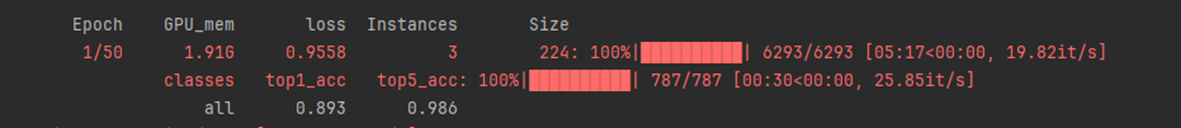
\includegraphics[width=1.0\textwidth]{img/train_yolo}
    \captionAuthorSource{Proces trénování YOLO11 modelu}
    \label{fig:train_yolo}
\end{figure}

Během trénování se sleduje výkonnost modelu na validačních datech, která zabraňují přeškolení.
Přeškolení si můžeme představit například u modelu, který rozpoznává kačeny, kočky a slepice.
I když všechny konfigurační parametry byly správně,  systém v některých případech špatně identifikoval kočku.
Až zpětnou analýzou trénovacích dat bylo zjištěno, že došlo k přeškolení.
Systém identifikoval kachnu nikoliv podle tvaru jejího těla, případně zabarvení, jako to udělá člověk, ale podle toho, zda na obrázku byla či nebyla tráva.
To pak vedlo k tomu, že pokud byla kočka na trávě, byla označena za kachnu.
Spustit trénovací smyčku je jednoduché.
Bylo třeba předat jen několik základních parametrů.


\begin{itemize}
    \item Epochs: 50 - znamená, kolik poběží učících cyklů
    \item Batch size: 16 - specifikuje, kolik vláken poběží paralelně, je třeba dbát na velikost paměti grafické karty
    \item Pretrained: True - říká, že budeme rozšiřovat již naučený model
    \item Data path: c:/kurnik/klasifikace/kurnik\_learn\_temp/train - specifikuje cestu odkud se načítají data k učení
\end{itemize}

\paragraph*{Krok 5 - YOLOTester:}

Po úspěšném tréninku modelu je nutné jeho testování na dříve oddělené testovací sadě.
Tento krok zahrnuje vyhodnocení výkonnosti modelu pomocí metrik, jako je přesnost, citlivost.
Testování nám poskytuje objektivní zpětnou vazbu o tom, co za objekty model umí ve snímcích rozpoznat.
Důležité je předkládat pro testování snímky, které během tréninku neviděl.
Na základě testovacích výsledků jsem pak následně prováděl úpravy učících parametrů, případně jsem dodával další data do učícího datasetu.

\begin{figure}[H]
    \centering
    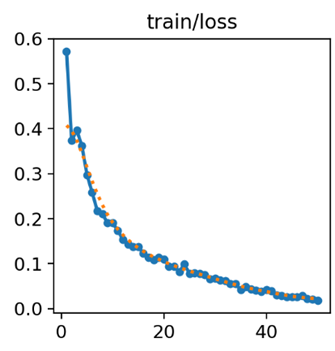
\includegraphics[width=0.5\textwidth]{img/loss_funkce}
    \captionAuthorSource{Graf loss funkce v závislosti na počtu etap}
    \label{fig:loss_funkce}
\end{figure}

Graf na obrázku~\ref{fig:loss_funkce}, který se při učení automaticky generuje, nám umožnuje sledovat, jak dobře se model učí vzhledem k časové ose tréninku.
Tento graf typicky zobrazuje ztrátovou funkci (loss) na svislé ose (Y) a počet trénovacích epoch nebo kroků na vodorovné ose (X).

\begin{figure}[H]
    \centering
    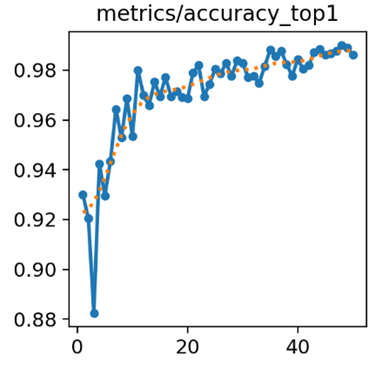
\includegraphics[width=0.5\textwidth]{img/top1_accuracy}
    \captionAuthorSource{Top-1 accuracy chart}
    \label{fig:top1_accuracy}
\end{figure}

Graf na obrázku~\ref{fig:top1_accuracy} se zaměřuje na metriku přesnosti, konkrétně na
"top-1 accuracy", která měří, jak často je nejpravděpodobnější (nejvyšší hodnocená) předpověď modelu správná.

Výsledky detekce jsou demonstrovány na obrázku~\ref{fig:detekce_slepic}.

\begin{figure}[H]
    \centering
    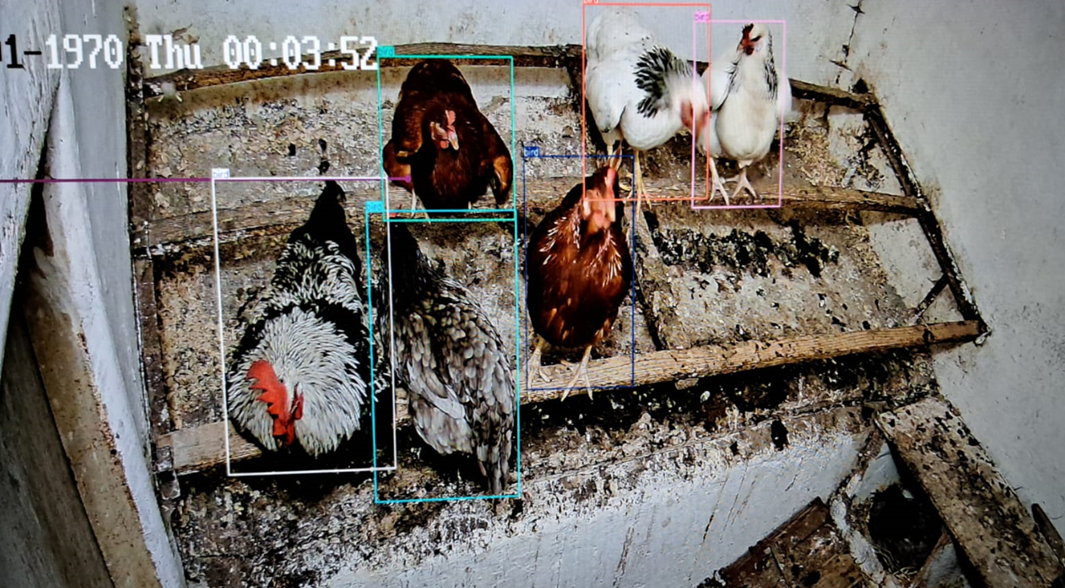
\includegraphics[width=0.8\textwidth]{img/detekce_slepic}
    \captionAuthorSource{Model detekující slepice}
    \label{fig:detekce_slepic}
\end{figure}
